
\documentclass[twocolumn]{article}
\usepackage{mathpazo}
\usepackage{microtype}
\usepackage{times}

 %%%%%%%%%%%%%%%%%%%%%%%%%%%%%%%%%%%%%%%%%%%%%%%%%%%%%%%%%%%%%%%%%%%%%%%%%%%%%
 %                              My Commands
\newcommand{\bi}{\begin{itemize}}
\newcommand{\ei}{\end{itemize}}
\newcommand{\be}{\begin{enumerate}}
\newcommand{\ee}{\end{enumerate}}
\newcommand{\ii}{\item}
\newtheorem{Def}{Definition}
\newtheorem{Lem}{Lemma}
\usepackage{algorithm}
\usepackage{algorithmicx}
\usepackage{algpseudocode}

\usepackage{graphicx}
\graphicspath{%
        {converted_graphics/}
        {./images/}
}
    
\setlength\textwidth{7in} 
\setlength\textheight{9.5in} 
\setlength\oddsidemargin{-0.25in} 
\setlength\topmargin{-0.25in} 
\setlength\headheight{0in} 
\setlength\headsep{0in} 
\setlength\columnsep{18pt}
\sloppy 
 
\begin{document}

\title{
\vspace{-0.5in}\rule{\textwidth}{2pt}
\begin{tabular}{ll}\begin{minipage}{4.75in}\vspace{6px}
\noindent\large Autonomous Control Middleware Research Section\\
\vspace{-12px}\\
\noindent\LARGE ETRI\qquad \large Technical Report 13VC1310-TR-01
\end{minipage}&\begin{minipage}{2in}\vspace{6px}\small
218 Gajeong-ro, Yuseong-gu\\
Daejeon, 305-700, South Korea\\
http:/$\!$/www.etri.re.kr/\quad 
\end{minipage}\end{tabular}
\rule{\textwidth}{2pt}\vspace{0.25in}
\LARGE \bf
How to Make a Technical Report (Rev. 3)
}

%\date{Autonomous Control Middleware Research Section, ETRI}

\author{
{\bf Sung-Soo Kim}\\
\it{sungsoo@etri.re.kr}
}

\maketitle

\begin{abstract}

The following document describes the preferred formatting of technical reports and submission guidelines.  This document itself is formatted according to the preferred formatting rules.

\end{abstract}

\section{Submission Guidelines}

The department accepts technical reports of various kinds.  In most cases the department's repository will display a description of the technical report, followed by a link to the report itself, plus an optional link to an archive of related data.  To submit a report, first contact the maintainer to get a technical report number, and then provide the maintainer with files as described below.

Technical reports are given unique numbers of the form {\bf GMU-CS-TR-\textit{year}-\textit{number}}.  {\it year} indicates the year in which the technical report was submitted, and {\it number} is the index numer assigned to the technical report for that year.

\begin{figure}[!t]
        \centering
        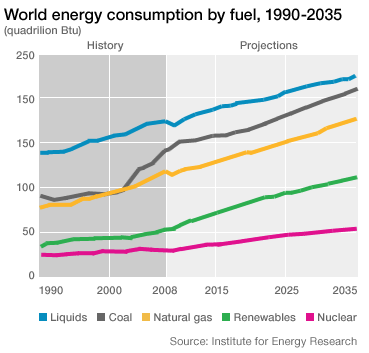
\includegraphics[width=0.33\textwidth]{test}
        \caption{Caption}
        \label{fig1}
\end{figure}



Format your technical report as described later in the document.  When you submit the report to the maintainer, it will consist of up to three files:

\begin{enumerate}
\item The report proper, ideally (but not required to be) formatted in a fashion similar to what you see here.  The report is in Adobe PDF and ends in {\tt .pdf}
\item A Bib\TeX \,entry of bibliographic information about the report: a plain text file ending in {\tt .bib}
\item An optional archive of associated data or code files.  An archive ending in {\tt .zip} which contains exactly one directory.
\end{enumerate}

Consult the technical report archive to determine who the current maintainer is.  At present, the archive can be reached from a link off of http:/$\!$/cs.gmu.edu/

\section{The Bib\TeX \,Entry}

We require a Bib\TeX \,entry in order to maintain a consistent bibliographic database of files online.  If you don't have experience in creating Bib\TeX \,entries, you may ask the technical reports maintainer for help, but first try to find someone else who understands Bib\TeX \,if you can.  

Bib\TeX \,files are simple text files which end in {\tt .bib}  The Bib\TeX \,entry for the document you're reading is shown below (you don't have to wrap the abstract this tightly):

\vbox {\scriptsize
\begin{verbatim}@TechReport{ GMU-CS-TR-2011-0,
   author =       { Sean Luke },
   title =        { How to Make a Technical Report (Rev. 3) },
   institution =  { Department of Computer Science,
                    George Mason University },
   address =      { 4400 University Drive MSN 4A5,
                    Fairfax, VA 22030-4444 USA },
   year =         { 2008 },
   howpublished = { Available at http://cs.gmu.edu },
   number =       { GMU-CS-TR-2011-0 },
   abstract =     { The following document describes the preferred
                    formatting of technical reports and submission
                    guidelines.  This document itself is formatted
                    according to the preferred formatting rules. },
}\end{verbatim}}

\section{The Data Archive}


You can put whatever you like in the data archive accompanying your report. The data archive is optional.  However, you must provide an actual file, not a link to a file (we keep copies of everything in the technical report database for consistency).  In the archive accompanying the report you're reading we've included a template in \LaTeX2e.  We imagine that common things accompanying most technical reports might include computer code, graphical image data, collected databases, etc.

\section{Formatting a Technical Report}

Technical reports must be submitted as a single Adobe PDF file.  The preferred format for technical reports is a PDF file generated from \LaTeX2e, using Times Roman as the font, and with approximately the same style as the document you are now reading.  There are no citation style rules.  {\bf This is \textit{not} a required format: but it is strongly recommended.}

\paragraph{Submitting via \LaTeX2e}  In the archive accompanying this document, we have provided a \LaTeX \,template file you can use.  In case you can't get ahold of this template, we have printed it out verbatim in the column to the right.  Please compile on a modern \LaTeX2e system, using \textit{pdflatex} rather than \textit{latex}, as some older systems do not have font mapping properly handled and PDF font rendering comes out dotty when read on-screen.

\paragraph{Submitting via Word or OpenOffice}  Try to format your document to look as similar as possible to the one you see here.  Body text is two-column, fully-justified, 10-point Palatino.  The first paragraph of a new section or subsection is not indented.  New section titles consist of a 14-point empty line, followed by a 14-point bold line with the section title, followed by a 10-point blank line.  New subsection titles consist of a 12-point empty line, followed by a 12-point bold line with a section title, followed by a 10-point blank line.

\section{Intellectual Property}

At time of submission, you must have permission of the copyright owner  in order to place the report in the repository, and placement in the repository implies permission by that owner to distribute the work publically.  If at a future time you lose permission of the copyright owner, you must contact the repository maintainer and ask that the link be removed.  This most commonly happens when your report was accepted to a journal or book and you had to transfer copyright.  If so, amend your Bib\TeX \,entry to indicate where the report has now been published, inserting a {\tt note} field like this:

\vbox {\scriptsize
\begin{verbatim}note = { Published as: (2011) S. Luke, ``The Cool Paper'',
         Journal of Irreproducible Results 4:2, April 2011 },\end{verbatim}}

\noindent Are you the copyright owner of this paper?  If you wrote this paper in your capacity as a student, a faculty member, or a research assistant, then you likely own the copyright.  If you wrote this paper in your capacity as a teaching assistant, as a staff member, or if you did this work on behalf of GMU for a specific task requested by GMU, then GMU probably owns the copyright.

Are you the copyright owner of software associated with this paper?  Patentable software or work created using ``substantial use of significant university resources with considerable potential commercial value'' may be owned by GMU, but if you release the code as open source, GMU does not claim the work.  To be certain, ask the Office of Technology Transfer, who are also authorized to release GMU copyrights.

\section{The \LaTeX2e Template}

We recommend this template for your technical report.  It was used to produce the document you are reading.

\vbox{\scriptsize
\begin{verbatim}
\documentclass[twocolumn]{article}
\usepackage{mathpazo}
\usepackage{microtype}

\setlength\textwidth{7in} 
\setlength\textheight{9.5in} 
\setlength\oddsidemargin{-0.25in} 
\setlength\topmargin{-0.25in} 
\setlength\headheight{0in} 
\setlength\headsep{0in} 
\setlength\columnsep{18pt}
\sloppy 
 
\begin{document}

\title{
\vspace{-0.5in}\rule{\textwidth}{2pt}
\begin{tabular}{ll}\begin{minipage}{4.75in}\vspace{6px}
\noindent\LARGE Department of Computer Science\\
\vspace{-12px}\\
\noindent\large George Mason University\qquad Technical Reports
\end{minipage}&\begin{minipage}{2in}\vspace{6px}\small
4400 University Drive MS\#4A5\\
Fairfax, VA 22030-4444 USA\\
http:/$\!$/cs.gmu.edu/\quad 703-993-1530
\end{minipage}\end{tabular}
\rule{\textwidth}{2pt}\vspace{0.25in}
\LARGE \bf
PUT YOUR TITLE HERE (NOT IN ALL CAPS)
}

\date{Technical Report
PUT YOUR TECHNICAL REPORT NUMBER HERE
}

\author{
{\bf FIRST AUTHOR NAME}\\
FIRST AUTHOR EMAIL ADDRESS
\and 
{\bf SECOND AUTHOR NAME (AND SO ON)}\\
SECOND AUTHOR EMAIL ADDRESS
}

\maketitle

\begin{abstract}
YOUR ABSTRACT GOES HERE
\end{abstract}

PUT YOUR BODY TEXT HERE

\end{document}\end{verbatim}}

\end{document}
